\begin{flushleft}
Il seguente codice calcola valori, errori e rapporti tra gli errori usando le 2 function precedenti:
\lstinputlisting[language=matlab]{cap_5/es2/es2.m}
Come richiesto riportiamo i valori in forma tabellare:
\begin{center}
\begin{tabular}{|c|c|c|c|c|}
\hline
k & Errore Trapezi & Rapporto Trapezi & Errore Simpson & Rapporto Simpson \\
\hline
1 &  5.6706e-01 &  --- & 7.0308e-01 & --- \\
2 &  2.3483e-01 &  4.1412e-01 & 5.0212e-01 & 7.1417e-01 \\
3 &  5.6353e-02 &  2.3997e-01 & 3.1390e-03 & 6.2514e-03 \\
4 &  1.3274e-02 &  2.3556e-01 & 1.0853e-03 & 3.4574e-01 \\
5 &  3.2632e-03 &  2.4583e-01 & 7.3810e-05 & 6.8010e-02 \\
6 &  8.1229e-04 &  2.4892e-01 & 4.6819e-06 & 6.3431e-02 \\
7 &  2.0285e-04 &  2.4973e-01 & 2.9360e-07 & 6.2710e-02 \\
8 &  5.0699e-05 &  2.4993e-01 & 1.8365e-08 & 6.2551e-02 \\
\hline
\end{tabular}
\end{center}
Lo script precedente genera i grafici sottostanti:
%\begin{figure}[H]
%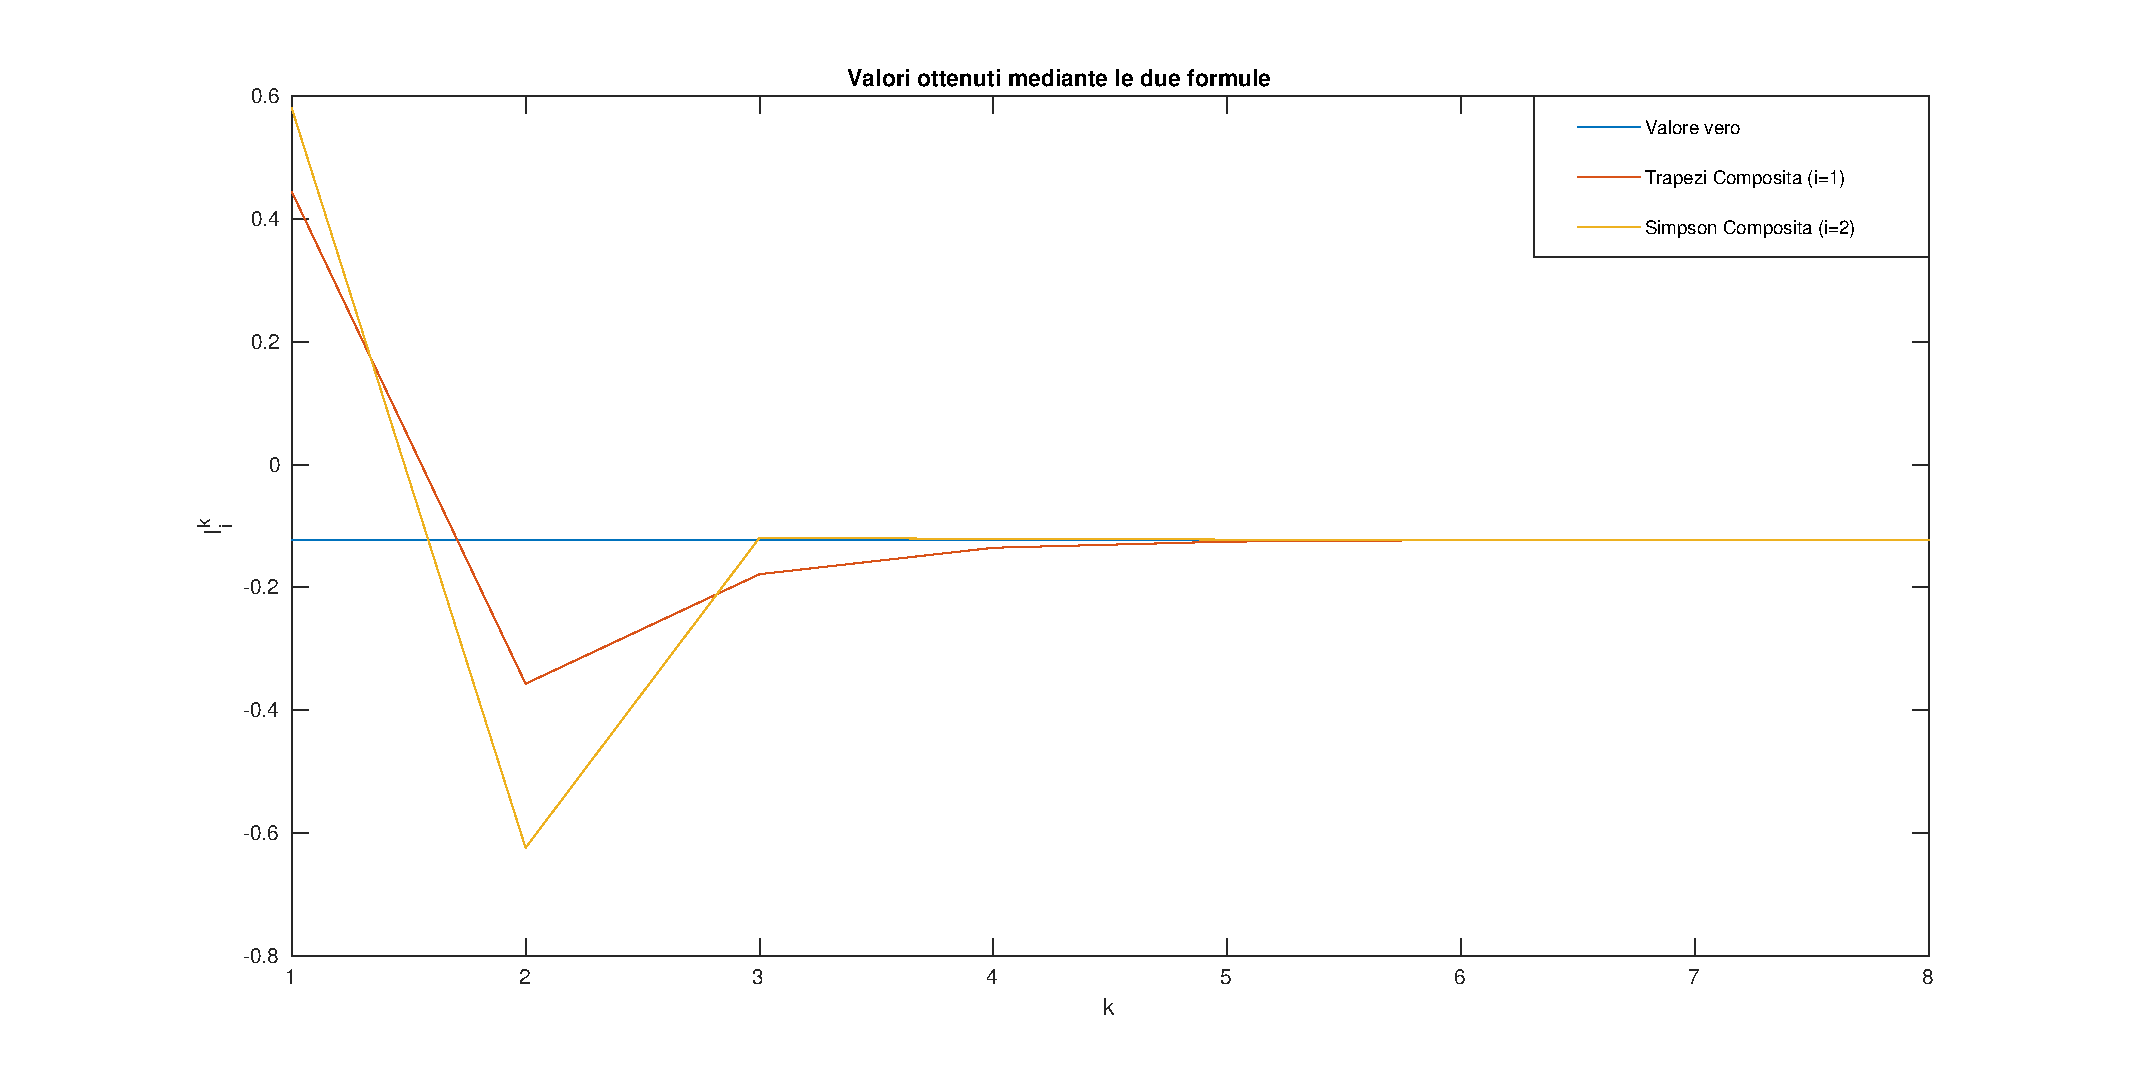
\includegraphics[width=480px, height=280px]{plot/fes52a}
%\end{figure}
\begin{figure}[H]
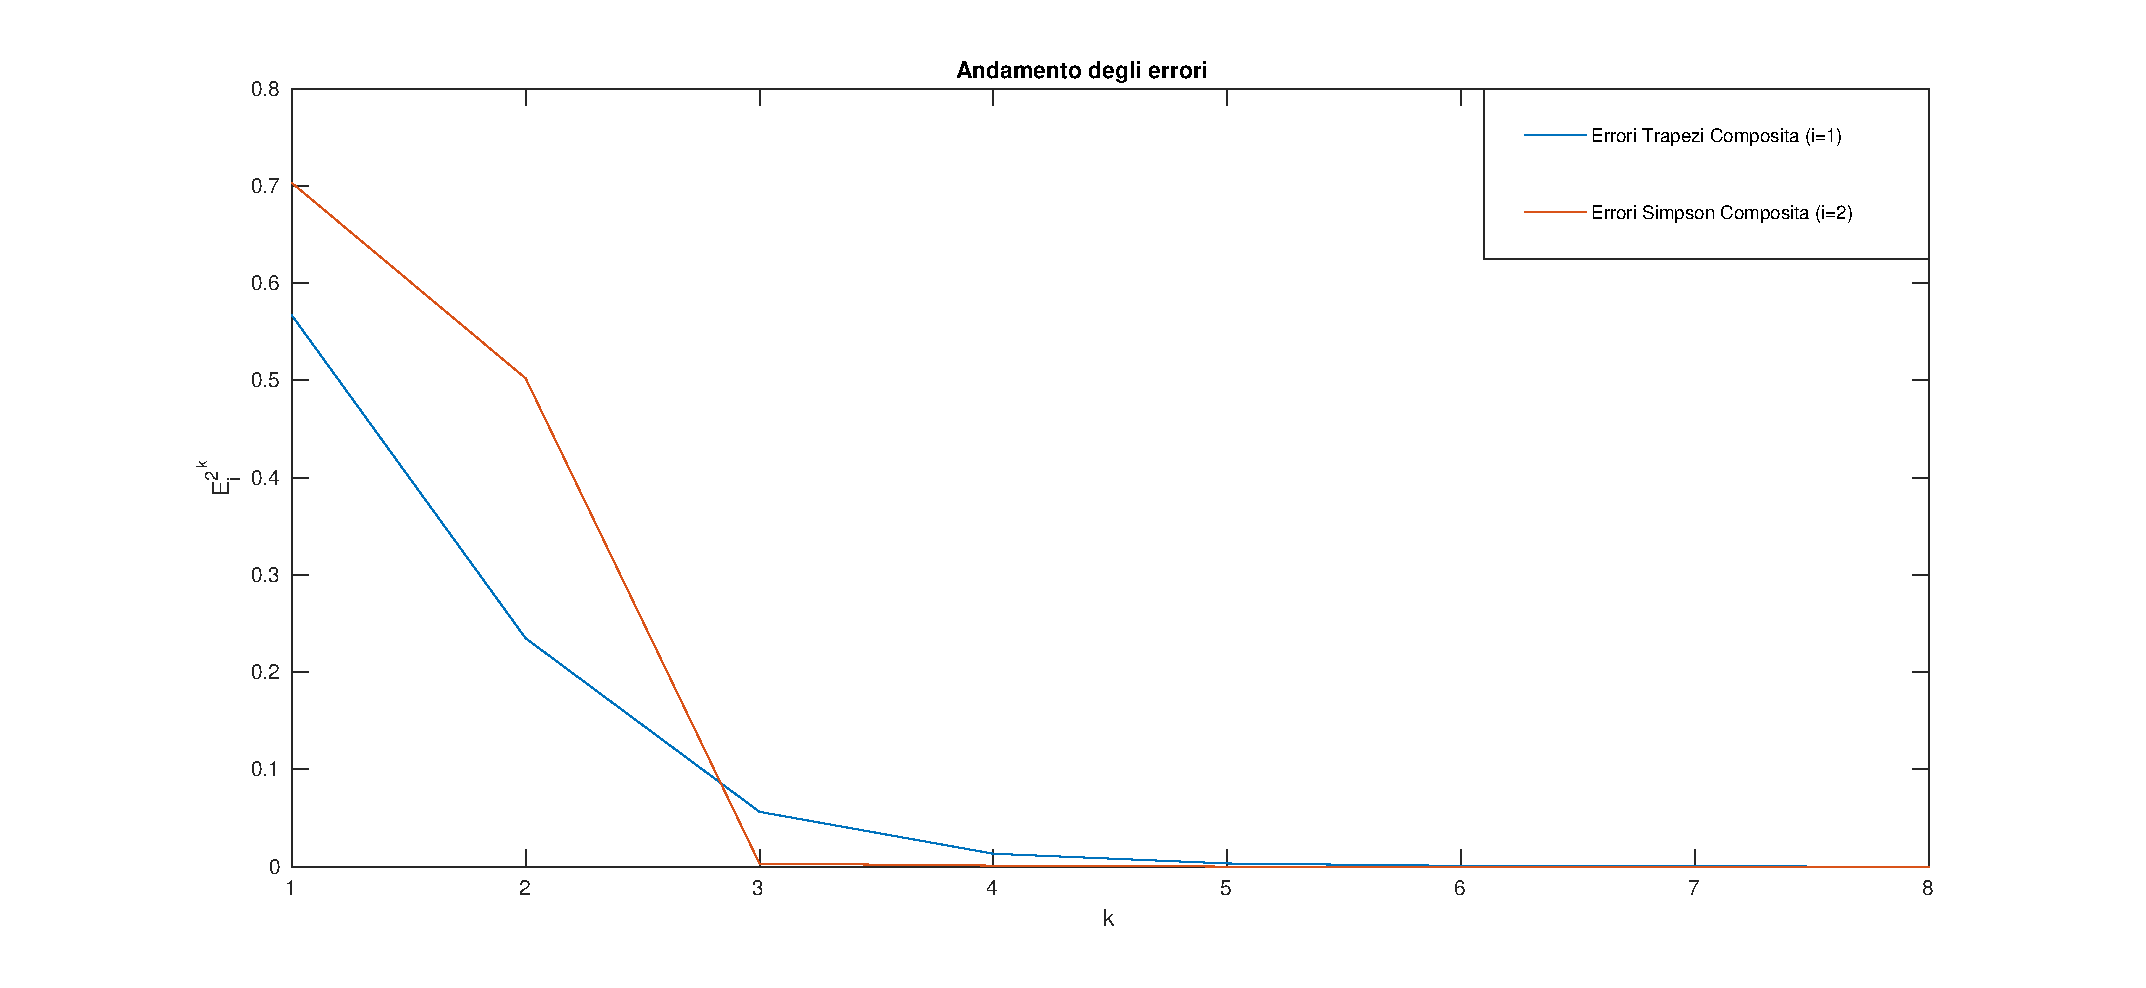
\includegraphics[width=480px, height=280px]{plot/fes52b}
\end{figure}
\begin{figure}[H]
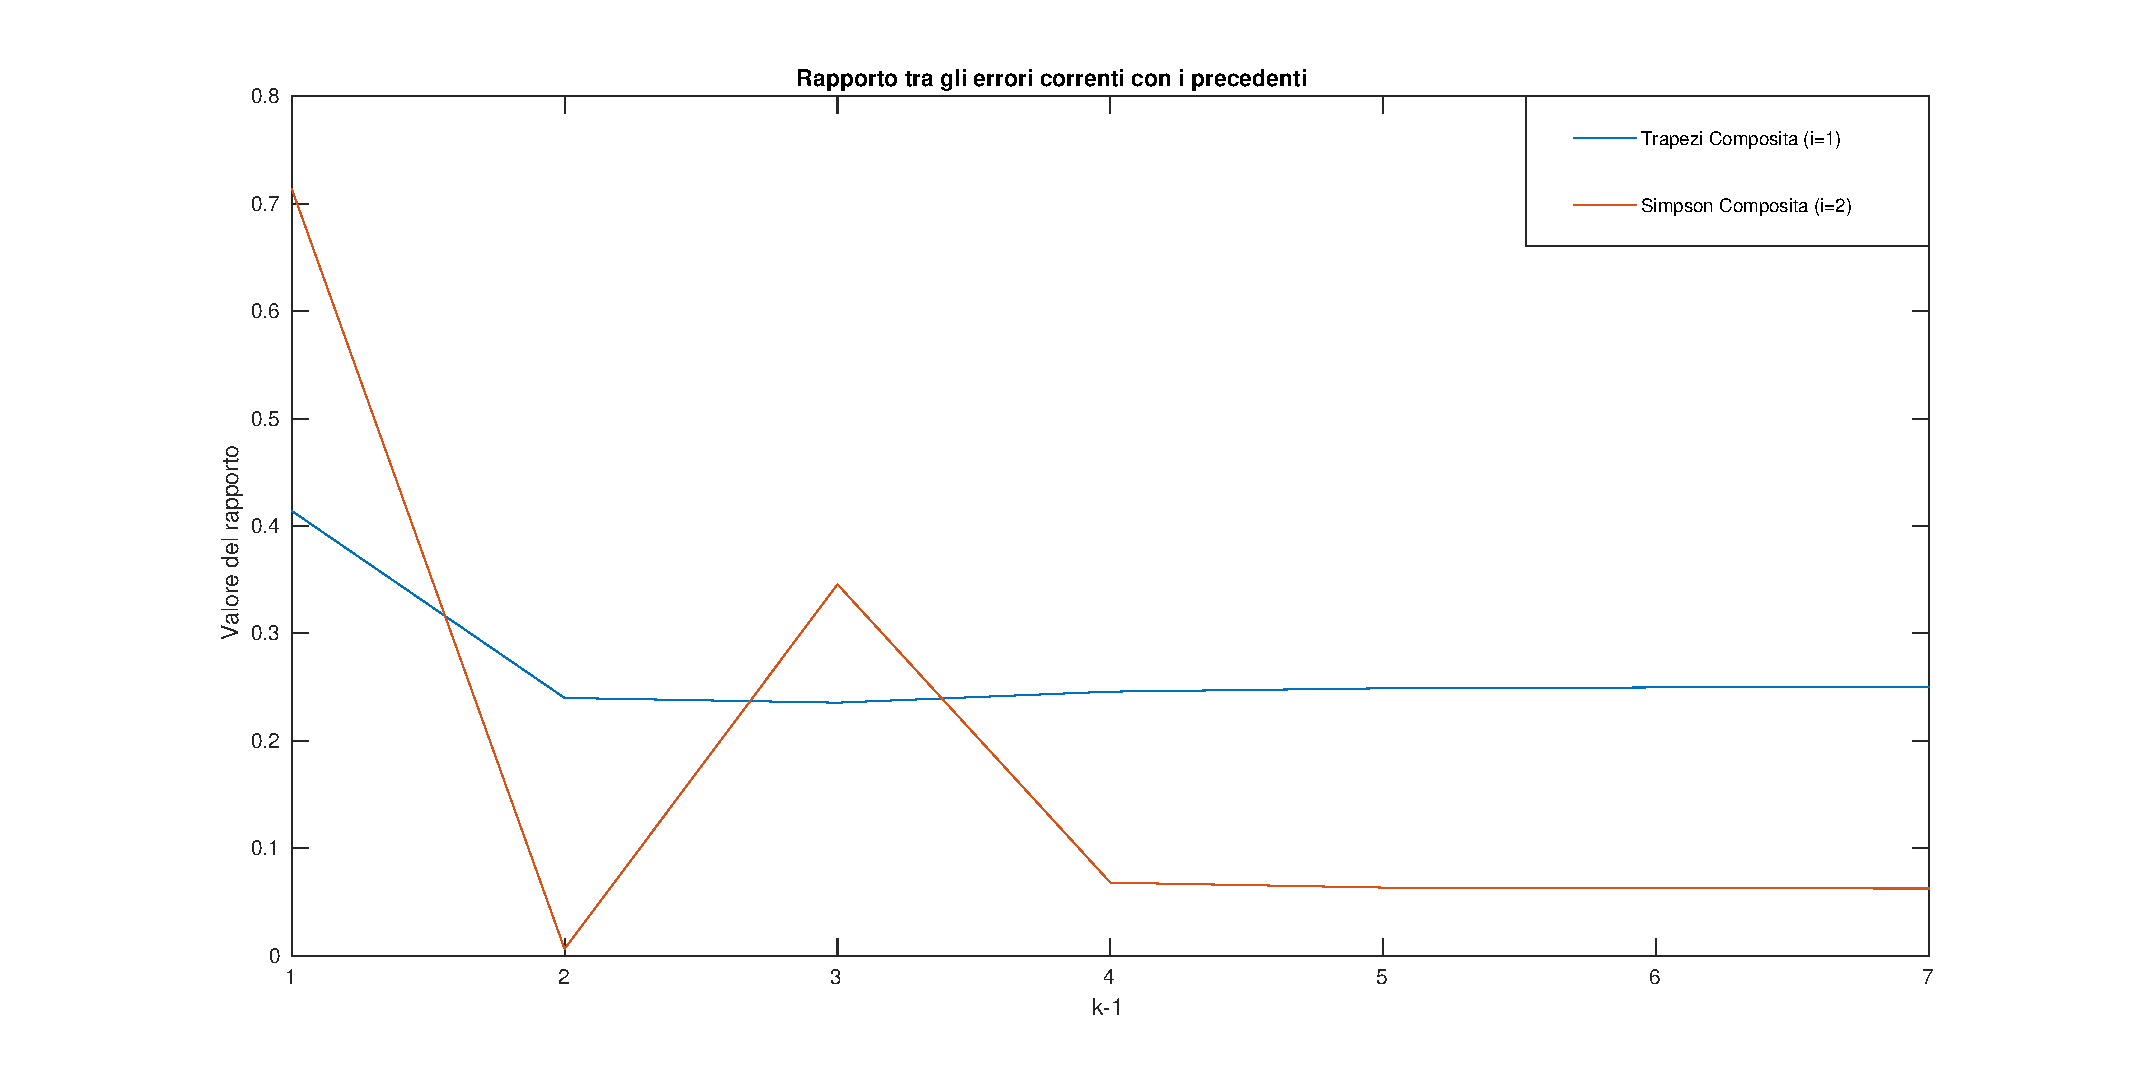
\includegraphics[width=480px, height=280px]{plot/fes52c}
\end{figure}
\end{flushleft}